\documentclass{article}
\usepackage[utf8]{inputenc}
\usepackage[english]{babel}
\usepackage{graphicx}
\graphicspath{ {images/} }
\usepackage{float}
\usepackage[T1]{fontenc}
\usepackage{amsfonts}
\usepackage{amsmath}
\usepackage{verbatimbox}
\usepackage{titlepic}
\usepackage{cite}
\usepackage{url}
\usepackage{geometry}
\usepackage{hyperref}
\usepackage{titling}
\usepackage{blindtext}
\usepackage{imakeidx}


 
\hypersetup{
    colorlinks=true,
    linkcolor=black,
    filecolor=black,      
    urlcolor=black,
}
\urlstyle{same}

\begin{document}
\font\myfont=cmr12 at 32pt

\begin{titlepage}

\title{\vspace{7ex} { {\myfont V2X - feature development}} \vspace{50ex} }
%
\includegraphics[scale=0.4]{images/titlepange.png}


\author{ Tedd Ahlberg, Erik Benjaminsson, Filip Kaiser \\ Fressia Merino,  Shahad Naji, David Olofsson}
\date{January 2019}
\end{titlepage}

%titel page no numbering  
\clearpage\maketitle
\thispagestyle{empty}

\cleardoublepage
\setcounter{page}{2}
\pagenumbering{Roman}			% Arabic numbering starting from 1 (one)
\setlength{\parskip}{0pt plus 1pt}


\Large{\textbf{Abstract}}
\\test

\newpage

% start index page 
\tableofcontents


\cleardoublepage
\setcounter{page}{3}
\pagenumbering{arabic}			% Arabic numbering starting from 1 (one)
\setlength{\parskip}{0pt plus 1pt}



\section{Introduction}
\subsection{Det här är en underrubrik? :)}
Backgroud - Vehicle-to-everything (V2X) communication is the passing of information from
a vehicle to any entity that may affect the vehicle, and vice versa. It is a vehicular
communication system that incorporates other more specific types of communication as 
V2I (Vehicle to Infrastructure), V2N (Vehicle-to-network), V2V (Vehicle-to-vehicle), V2P (Vehicle-to-Pedestrian), V2D (Vehicle-to-device) and V2G (Vehicle-to-grid) 
%́The main motivations for V2X are road safety, traffic efficiency, and energy savings.

Introduktion till ITS-G5, varför använda ?, var används den? vilken MHz(mer theory)
Tanken med V2X är att man skall få snabbare responstid än med cloud 

V2X utvecklas för att minska olyckor i trafiken, det finns olika typer av V2X\bigskip



V2X is short for vehicle-to-everything, it is meant to make traffic safer by letting the car communicate with surroundings and make the driver more aware. There is different types of communication such as V2I (vehicle to infrastructure), V2G (vehicle to grid), V2D (vehicle to device), V2V (vehicle to vehicle), V2P (vehicle to pedestrian) and V2N (vehicle to network). In this project we will focus on a special case of V2I where a moving car moving towards a crossing is simulated, to understand risks and problems. ITS-G5 will be used as a communication protocol, it is a standard wifi connection. Because standard wifi is already tested, widely implementable and cheap it can be used for safety in vehicles. To simulate access point (wifi) a software osCar is used and implemented in a simulation environment called otto
\section{Background}
The background for this project is to create safer travelling systems for all actors on the market. By bike, by feet or by car does not matter since the vision is that 0 casualties should occur in a traffic accident.\bigskip

Therefore a system that communicates with cars, infrastructures or other vehicles to lower the percentage of fatal accidents are very sought after, and vehicle manufacturers have been developing this technology for a long time the problem they have now are latency since the existing system depends on a cloud service which has too long latency in some situations where a microsecond could make a big difference.
\section{Theory}
\subsection{Det här är också en underrubrik}
\subsubsection{Det här är underrubrikens rubrik}
In today's automotive companies huge resources are put in optimising and developing efficient processes that are in favour of the environmental, safety on the roads and antonyms cars. In this cluster of new technology is something called "V2V" \textit{(Vehicle-to-vehicle communication)}. V2V is a wireless transmission system between cars on the road. The reason and idea behind this technology is to get cars around each other to communicate with each other to reduce the risk of both collision and more energy effective driving. The information that is sent between the cars are their speed, position and direction.

\begin{figure}[H]
    \centering
    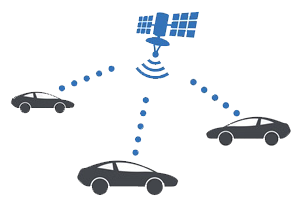
\includegraphics{images/V2VGlobal.png}
    \caption{Cloud network}
\end{figure}


This information is sent over an AD-HOC [reference] network. AD-HOC is a local area network (LAN) that's used in close area networking. This is used instead of a global network “cloud network”. 

\begin{figure}[H]
    \centering
    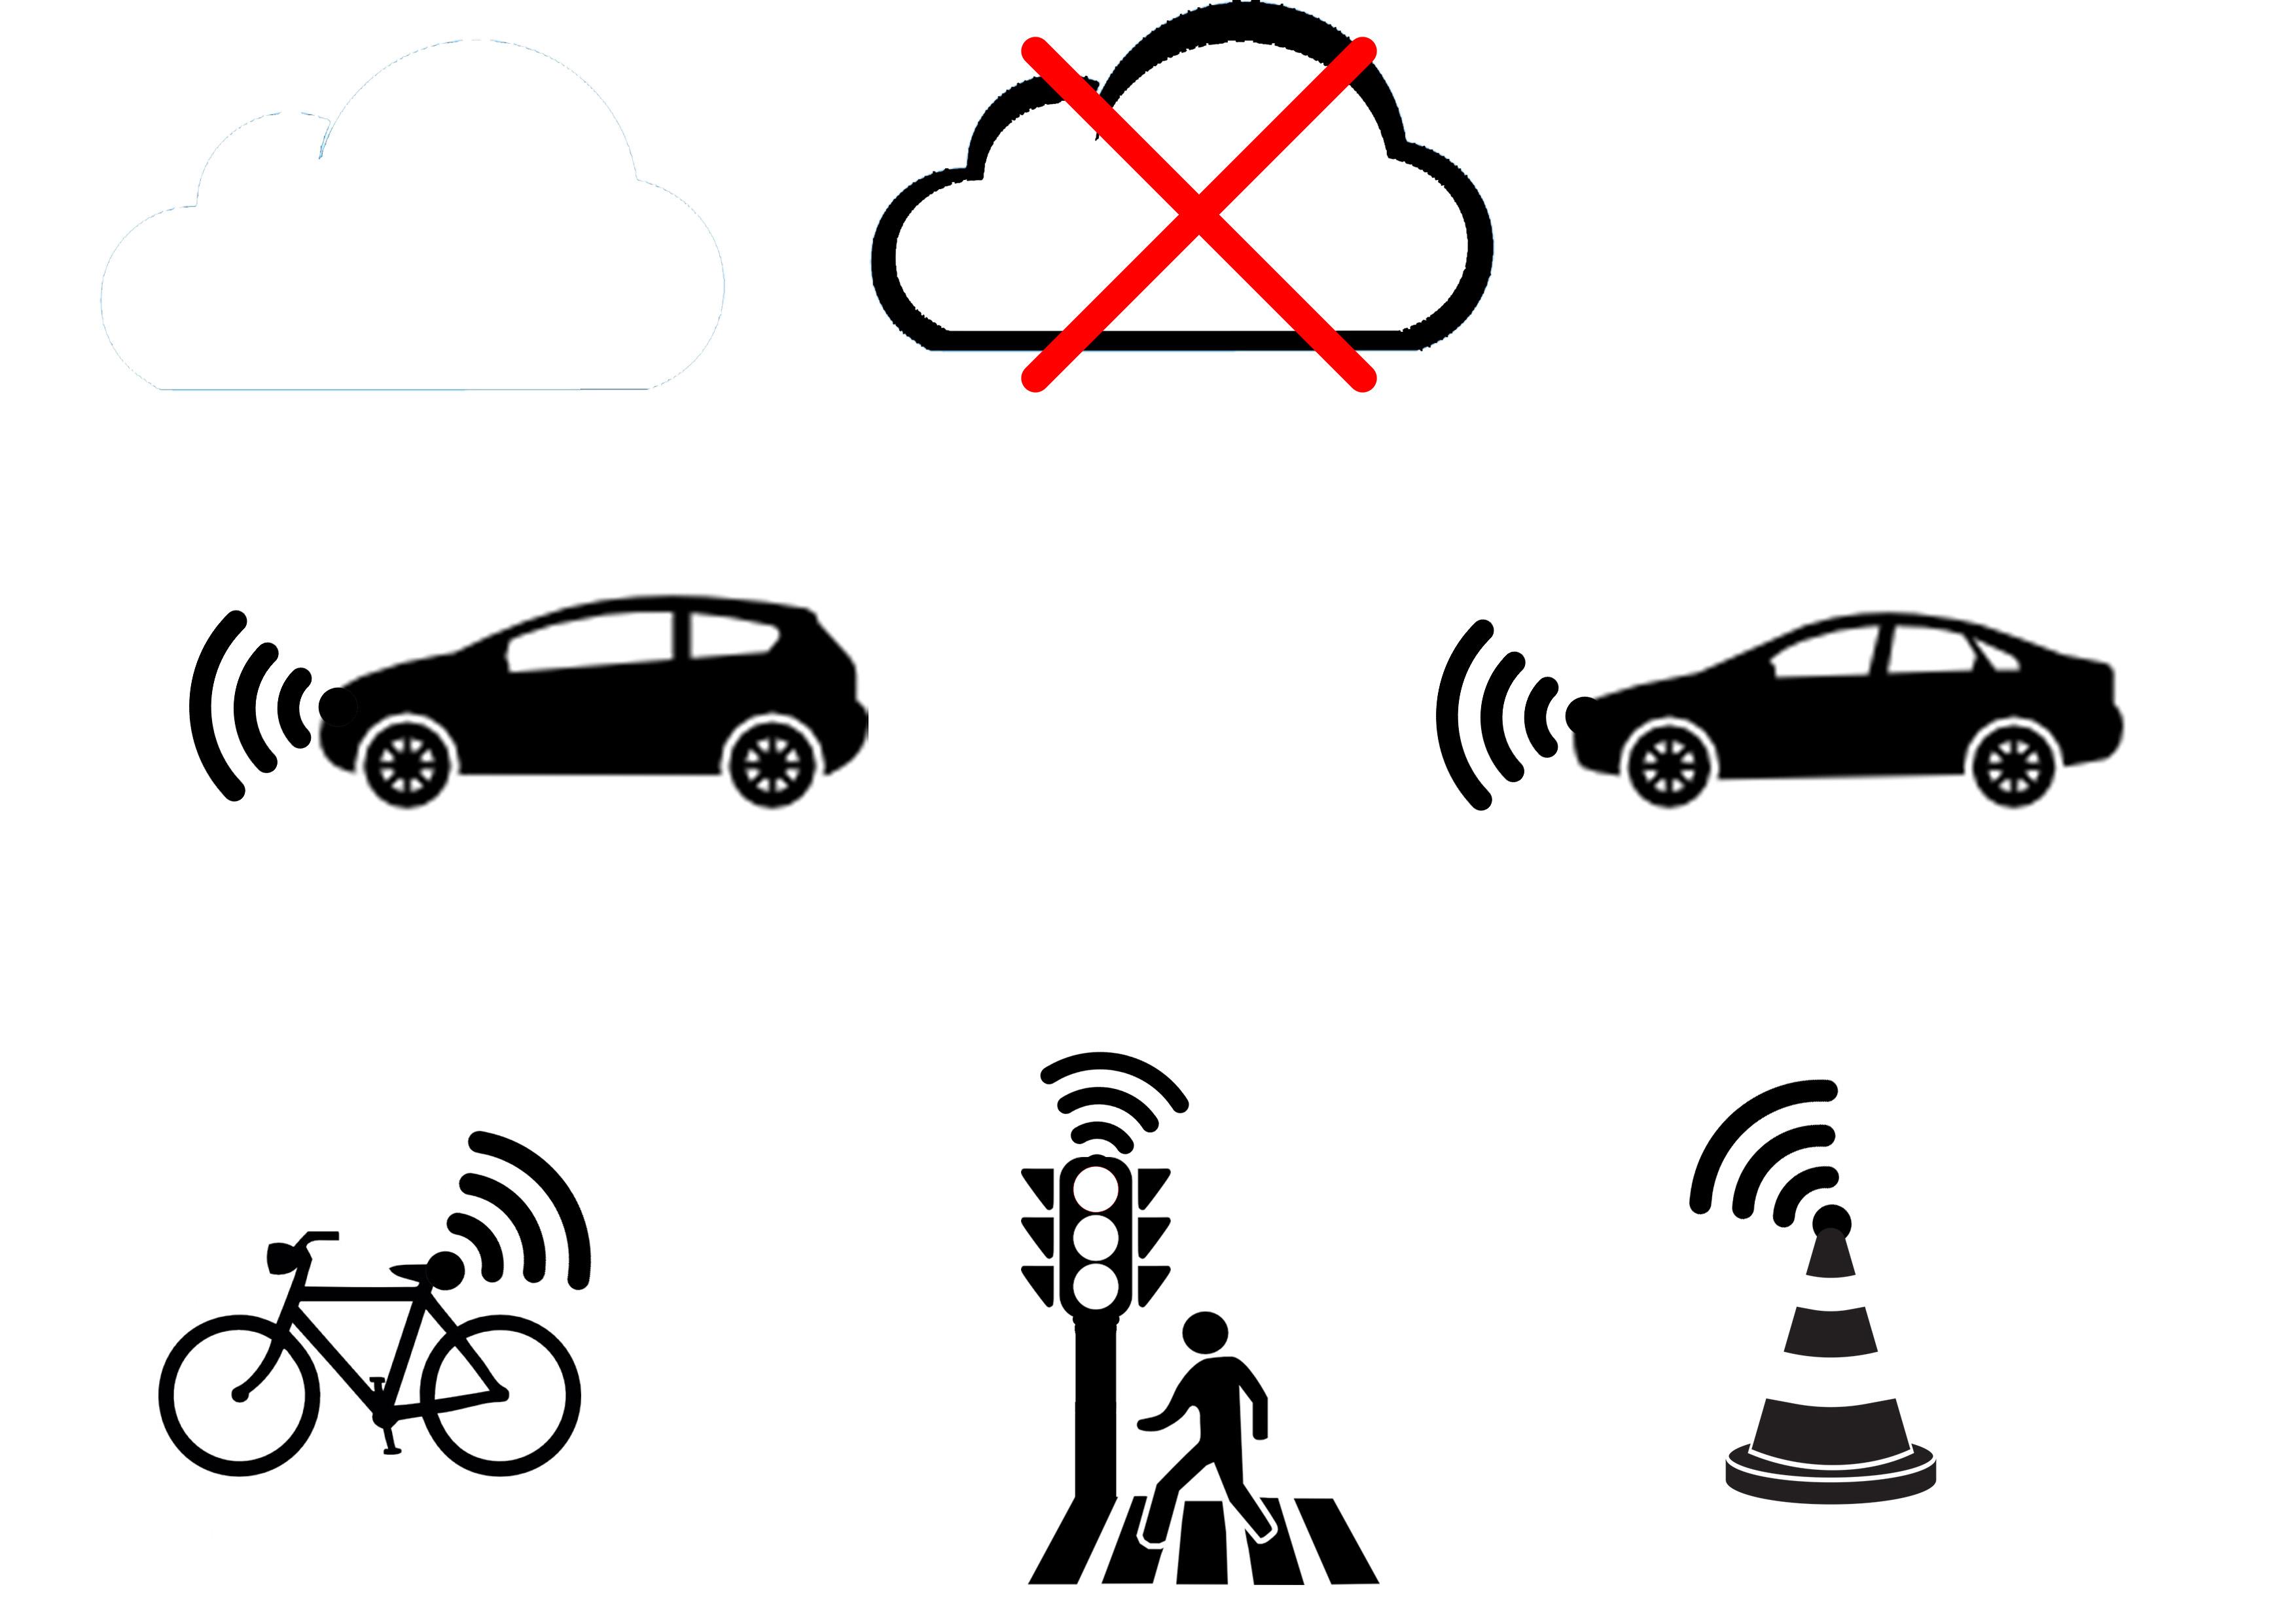
\includegraphics[scale=0.4]{images/projektsketch.jpg}
    \caption{LAN network}
\end{figure}

AD-HOC is used for many reasons but mostly because a global network can have delay between the server and the cars and is hard to use in areas with bad connection to the grid. By using AD-HOC the delay in the signals between the vehicles are reduced and in traffic a shorter delay can save lives.
\bigskip

The goal of V2V is to reduce the total of cars crashes and especially in the future when cars are becoming completely autonomous and driving by themselves. This is where the V2X project enters the picture, \textit{"Because if cars are to communicate with each other, why not let the cars communicate with everything on the road like bikes, traffic lights and pedestrian crossings. Is that possible?"} It had reduced the risk of collision even more.
\bigskip

The technology used is called "Cooperative Intelligent Transport Systems" (C-ITS).  “ITS-G5” is a broadcast technology based on an evolution of the wireless standard 802.11p. It is the only validated and available technology on the market and capable of delivering secure AD-HOC direct vehicle-to-vehicle and/or vehicle-to-infrastructure communication. ITS-G5 is running in the designated 5.9 GHz frequency band that is foreseen for road safety. We emphasise that all technologies that run in this frequency band should not cause interference with each other and be interoperable.C-ITS should be able to demonstrate its capability to co-exist with electronic road charging, the enforcement of drive and rest times and weights and dimensions on the adjacent 5.8 GHz frequency band. [reference]

\section{Method}

%\bigskip 
%ger stort mellanrum \medskip ger lite mindre mellanrum \smallskip ännu mindre
%\paragraph{Här skriver man vad sin paragraph ska heta, det används mer då man vill dela upp sin text i olika delstycken typ om man ska förklara elektriska komponenter så blir varje delstycke en komponent 


\paragraph{}
The administration of the project was composed of a conjoint Google Drive storage sharing, Trello application for task planning and management together with the application Slack for all the communication.

It was decided that the group would have a minimum of two meetings a week, at the beginning and end of each week, to review and discuss the work done so far along with planning goals and tasks for the upcoming week. At the end of each week, the group would try to have a meeting with the supervisor at Cybercom, where he would review the progress of the project, answer questions from the group members and give advise or help with the program software. Other project related questions and problems were directed to the Chalmers' supervisor, who has been helping with the way to plan and organise the project for us to be able to complete it in time.

\paragraph{}
Before getting access to anything from the company all group members signed a standard non-disclosure agreement because the software that was going to be handed out to potentially be worked with contained confidential information. The group members also got access to the company's Github account with relevant information about the project. We received a log file with annexed documentation, to be parsed. 

\paragraph{}
The group decided on a specific case scenario to solve and with the help of Scrum the case was broken down into smaller, more feasible tasks. 

Our original method to test our V2X scenario was supposed to use the software supplied by Cybercom, but after some weeks we had to rethink our plans. The new strategy was to create a database with which to parse the information we acquired from the pseudo-log file with the purpose to map the locations of the two entities registered in the file and study the gathered data at each point. 

\paragraph{}
To achieve this a database schema was costructed capable of holding the data and a parser to read the log into the databas was written in java according to the following methodology.

By mapping each value on the line with its ID as key in a hashmap the data for each column in the database is parsed as it is found. This handles all the top-level IDs but needs special adjustment for the "location" and "blackboardProperties" entries.

By splitting the "location" entry into "longitude" and "latitude" in the line's hashmap it is handled with the rest.

Storing "blackboardProperties" requires more adjustments, since there can be any number of entries per line. To manage this a separate database table holds the property entries. The number of the parent line is entered as the identifier for the parent line and the data in the line's hashmap is inserted into the database when reaching "blackboardProperties"; since it is the last  type, not stored with the rest and depends on the parent line existing in the database (as seen in the database schema). In "blackboardProperties" the data for "type" and value (ID varies) are inserted into a new hashmap with their IDs as keys. Each "blackboardProperties" entry is inserted into the database when fully read. It is entered with the line number of the parent as "parent", value of "type" as "type" and the value of the remaining key (key ignored) as "value".

Thus, when reaching the end of the line all data has been parsed and inserted into the database.


\section{Results}

Coming in a few weeks (aiming for week 49/50)

\section{Discussion}
For future work it is recommended to have documents, such as documentation about the project and NDA:s, prepared and ready for the first meeting with the assigned group and to have the software ready to be handed out. That would have helped the speed and progress of the project. Though, as mentioned before, with the circumstances that we had we think that our achievement is a good start for farther development of the V2X research. 
\paragraph{}
We chose not to create a test program based on out assumptions about the software without taking a look at it and without knowing its structure and what information we could receive. Instead we decided to focus on writing theoretically about the techniques of V2X and creating a database that simplifies the assessing of information from the log-file that we got from Cybercom and potentially easing the way for future developers to analyse this kind of information.

\paragraph{}
The time distribution was a problem mostly because it was very difficult for us to get the files and the program that we initially planned to work with. When we finally got the files that we needed there was little time left for us to analyse it and work on our scenario, which resulted in adding more limitations to our work, by scoping down to focusing on parsing the log file into a database. This caused our work to be very theoretical instead of being practical like we had planned from the start. We were anticipating from the start to have access to OTTO to be able to simulate a test to develop a basic implementation of our case scenario. Therefore, as we mentioned in the result, we were only able to create a database and construct a basic implementation which stores information from the log file in a database. 

\paragraph{}
The cooperation between all the group members in the project worked well and we did everything that we could to create something useful with the available material. There were some areas of improvement in some aspects such as time planning and work distribution because it was our first time working with this type of project so it was a little hard to know how to organise the work and set up a working schedule that fits all group members. 




\section{Conclusion}

Our purpose was to make a pilot-study for future development of V2X technology. We chose to create a database into which we parse information from a log-file given to us by Cybercom. This enables filtering and searching for specific data in the future development of the project. The next step of this project would be creating a program to visualise the data which would give a clearer understanding of what that data signifies. 
\paragraph{}
We were not able to simulate our hypothetical scenario because of the short time-span of the project and administrative issues (permits) with OsCar and OTTO, which was part of our original plan. But through our theoretical investigation and assumptions we can conclude that this is a promising project for students as a thesis work, since the concept behind V2X could be an implementable feature in upcoming projects. If we would to recommend this project as a thesis work for students, it would be necessary to have access to the software provided by Cybercom which is required to be able to test their theories in OsCar and OTTO. With the database that we created, it will be easier for future developers to understand the log-files and be able to read the information easier. With some modifications to the script you could visualise that information to help with building your own test scenarios. It would also be helpful to have a set Gantt-scheme to organise and structure the workload and set up smaller deadlines to test the implementations of V2X scenarios. 
 



\newpage
\paragraph{References}
\begin{verbatim}
[1] - Documentation on \textit{ITS-G5 is ready to roll}, Available:
      https://itsg5-ready-to-roll.eu/} [Accessed: 10-11-18] 

[2] - From Wikipedia, the free encyclopedia, \textit{Local area network}, Available: 
      https://en.wikipedia.org/wiki/Local_area_network [Accessed: 28-11-18] 

[3] - From Wikipedia, the free encyclopedia, \textit{Wide Area Network}, Available: 
      https://sv.wikipedia.org/wiki/Wide_Area_Network [Accessed: 28-11-18] 

[4] - Cybercom Group a IT consulting company, Available:
      https://www.cybercom.com/sv/ [Accessed: 01-11-18]
\end{verbatim}

\newpage
\section{Appendix}
[1] - https://itsg5-ready-to-roll.eu/

\end{document}


%lite kommentarer
%i conclusion börja kanske inte vad man inte kunde klara av, 
%skriv typ, syftet var såhär och sen komma in på vad vi inte klarade av, även vad vi har klarat av. osv

%visa mer i resultat i resultat, skriv vad man hade kunnat göra med datan
%beskriv koden, referera till den i appendix, hur ser 

%diskussion, vilka var limitations? skriv mer så att någon annan förstår

%conclusion vilka papers? -kontrakt, dokumentation osv

%resultat-hur går man vidare?

Jens:

hur går man vidare?

hur tycker vi att det var att börja med projektet? hur har det känts?